\documentclass[12pt,a4paper, titlepage]{article}
\usepackage{amsmath}
\usepackage{graphicx}
\usepackage{float}
\usepackage{wrapfig}
\usepackage[russian]{babel}
\usepackage[utf8]{inputenc}


\title{Лабораторная работа 5. Решение задачи Дирихле для уравнения Пуассона методом установления. Вариант 2}
\date{2021\\Май}
\author{Петраков Иван\\\ МФТИ\\\\\\\\\\\\\\\\\\\\}
\hoffset = 0pt
\voffset = 0pt
\textheight = 700pt
\topmargin = 0pt
\headheight = 0pt
\headsep = 0pt
\marginparwidth = 0pt
\oddsidemargin = 0pt
\textwidth = 450pt

\begin{document}

\maketitle

\subsection*{Описание задачи}
\noindent\rule{\textwidth}{1pt}
Имеем задачу Дирихле для уравнения Пуассона:
\begin{equation}
\begin{cases}
\frac{\partial^2u}{\partial x^2} + \frac{\partial^2u}{\partial y^2} = -25 \pi^2 sin(3 \pi x)sin(4 \pi y) |
\\
u|_{\text{Г}} = 0
\end{cases}
\end{equation}
\\
x и y заданы на отрезке от 0 до 1.
\subsection*{Аналитическое решение}
\noindent\rule{\textwidth}{1pt}
Аналитическое решение можно подобрать, заметив, что можно искать решение в виде $u = a\cdot sin(3\pi x)sin(4\pi y)$. Тогда, подставив решение в таком виде в исходное уравнение, найдем, что $a = 1$. Итоговое аналитическое решение есть $u = sin(3\pi x)sin(4\pi y)$.

\subsection*{Программная реализация и практические исследования}
\noindent\rule{\textwidth}{1pt}
В качестве разностной схемы рассмотрим:
\begin{equation}
\begin{cases}
\frac{u^{n+1}_{l, m} - u^n_{l, m}}{\tau_n} = \frac{u^n_{l+1, m} - 2 u^n_{l, m} + u^n_{l-1, m}}{h_x^2} + \frac{u^n_{l, m+1} - 2 u^n_{l, m} + u^n_{l, m-1}}{h_y^2} + 25 \pi^2 sin(3\pi x)(sin(4\pi y)
\\
l = 1, 2, ..., L-1, m = 1, 2, ..., M-1, n = 0, 1, ..., N
\\
u^0_{l, m} = \psi_{l, m}, l = 0, 1, ..., L, m = 0, 1, ..., M
\\
u^n_{0, m} = u^n_{L, m} = u^n_{l, 0} = u^n_{l, M} = 0, l = 1, 2, ..., L-1, m = 0, 1, ..., M, n = 0, 1, ..., N
\end{cases}
\end{equation}
Здесь $\psi$ - произвольная функция, определенная в области интегрирования. Для удобства зададим ее равной нулю.
\\
\\
Определимся с оптимальными шагами по времени. Они задаются следующим выражением:
\begin{equation}
	\tau_n = \frac{2}{2 \pi^2 + 4(L^2+M^2) + [4(L^2+M^2) - 2 \pi^2] cos(\frac{\pi(2 n - 1)}{2 N})}
\end{equation}
\\
\\
Для придания устойчивости необходимо изменить порядок следования элементов в полученной последовательности $\tau_n$. Как это сделать - написано в предложенной к лабораторной работе литературы. Здесь же будет приведена итоговая последовательность с измененным порядком для каждой тройки L, M, N.
\\
\\
В нашем случае, ошибка $\epsilon$ задана равной $10^{-4}$. Для придания устойчивости N оценивается как 
\begin{equation}
	N >= ln(\frac{2}{\epsilon}) / ln\frac{\sqrt{4(L^2+M^2)} + \sqrt{2 \pi^2}}{\sqrt{4(L^2+M^2)} - \sqrt{2\pi^2}}
\end{equation}
\\
Поэтому, задавая набор L, M мы сразу определяем и необходимое значение N, и набор $\tau_n$.
\\
\\
Перейдем к расчетам. Их будем проводить на последовательно удваеваемых сетках L = M, начиная с L = 5, заканчивая L = 320.
\begin{figure}[H]
	\centering
	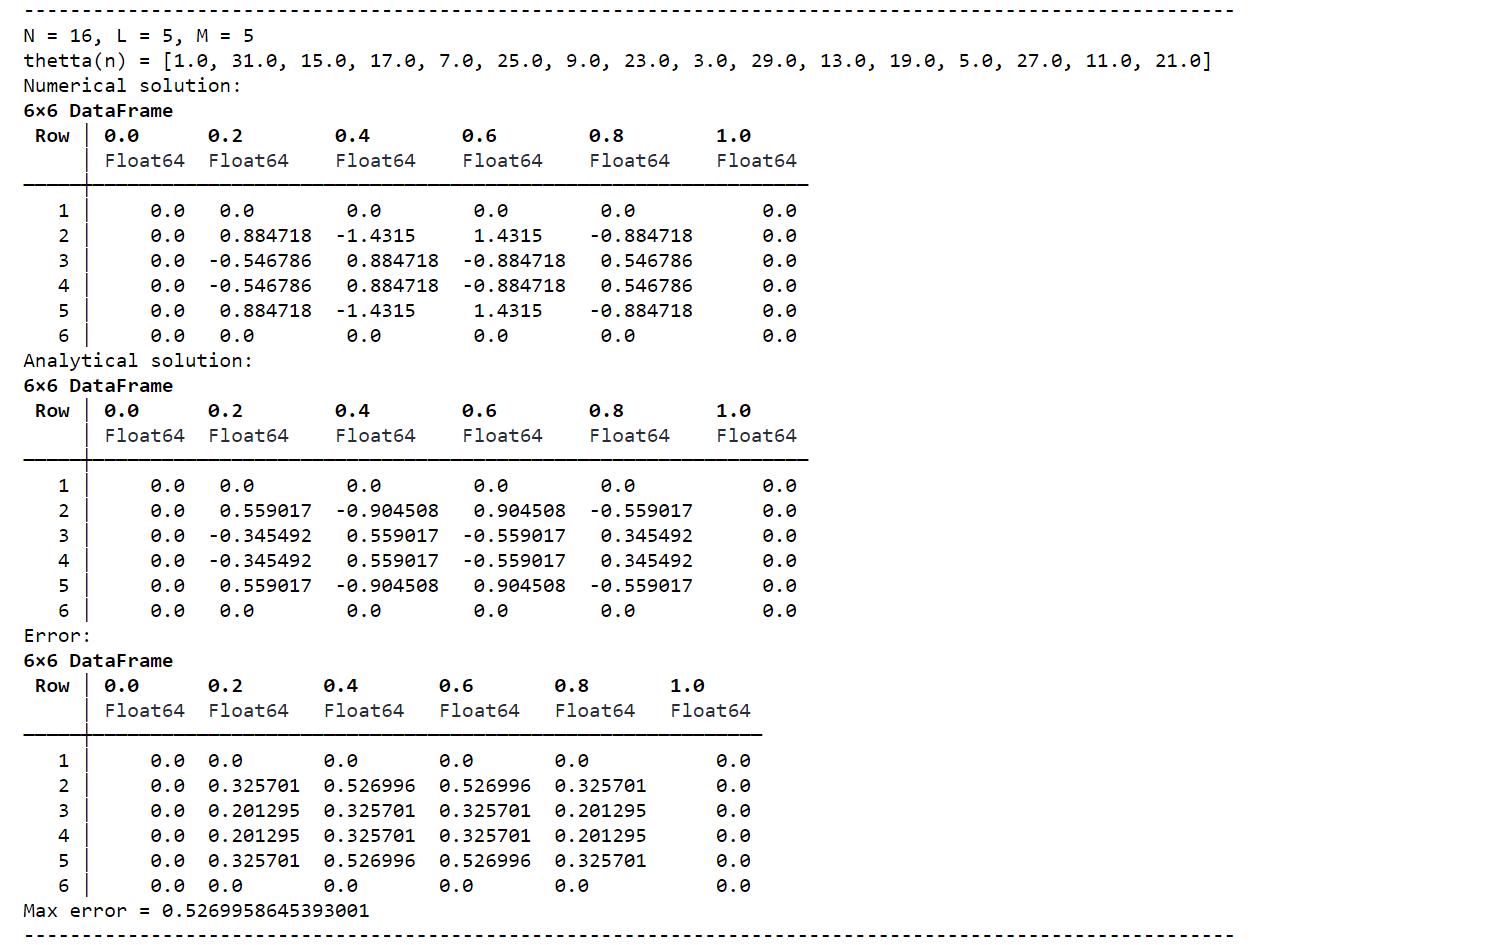
\includegraphics[width = 1.0\textwidth]{lab_5_0.png}
\end{figure}
\begin{figure}[H]
	\centering
	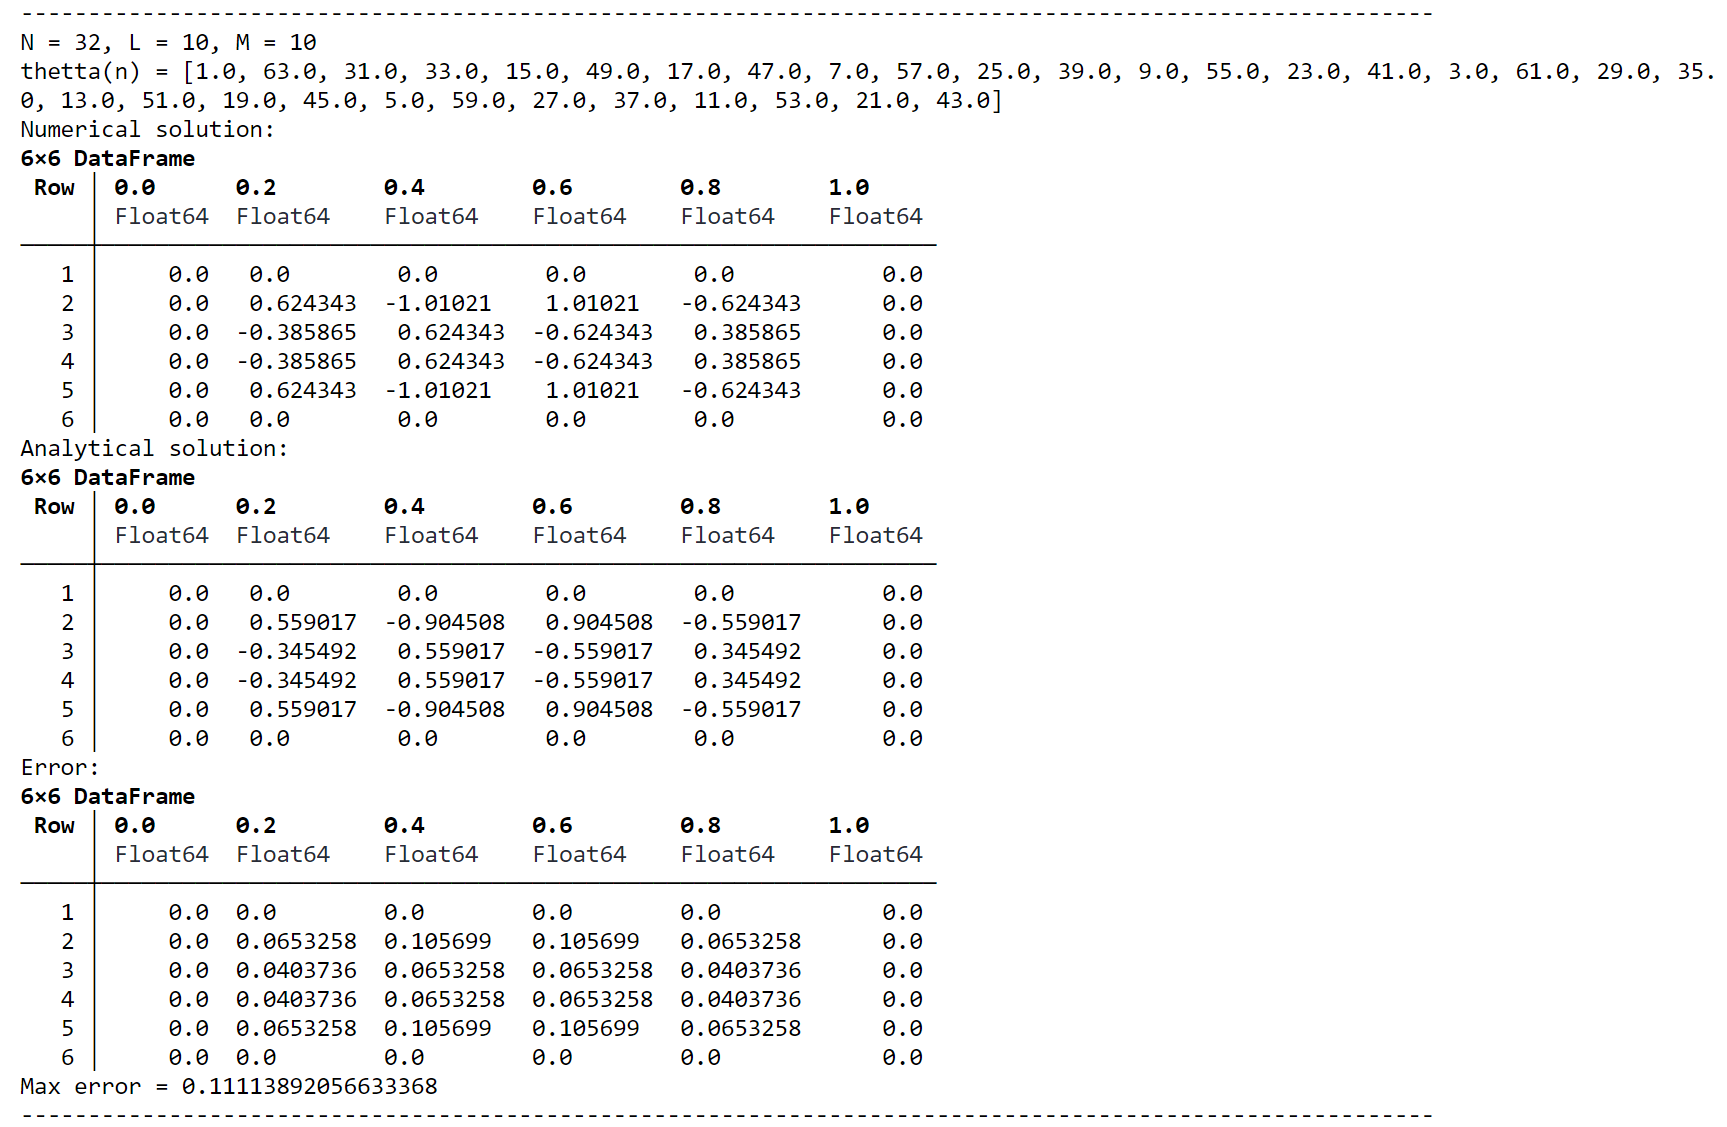
\includegraphics[width = 1.0\textwidth]{lab5_1.png}
\end{figure}

\begin{figure}[H]
	\centering
	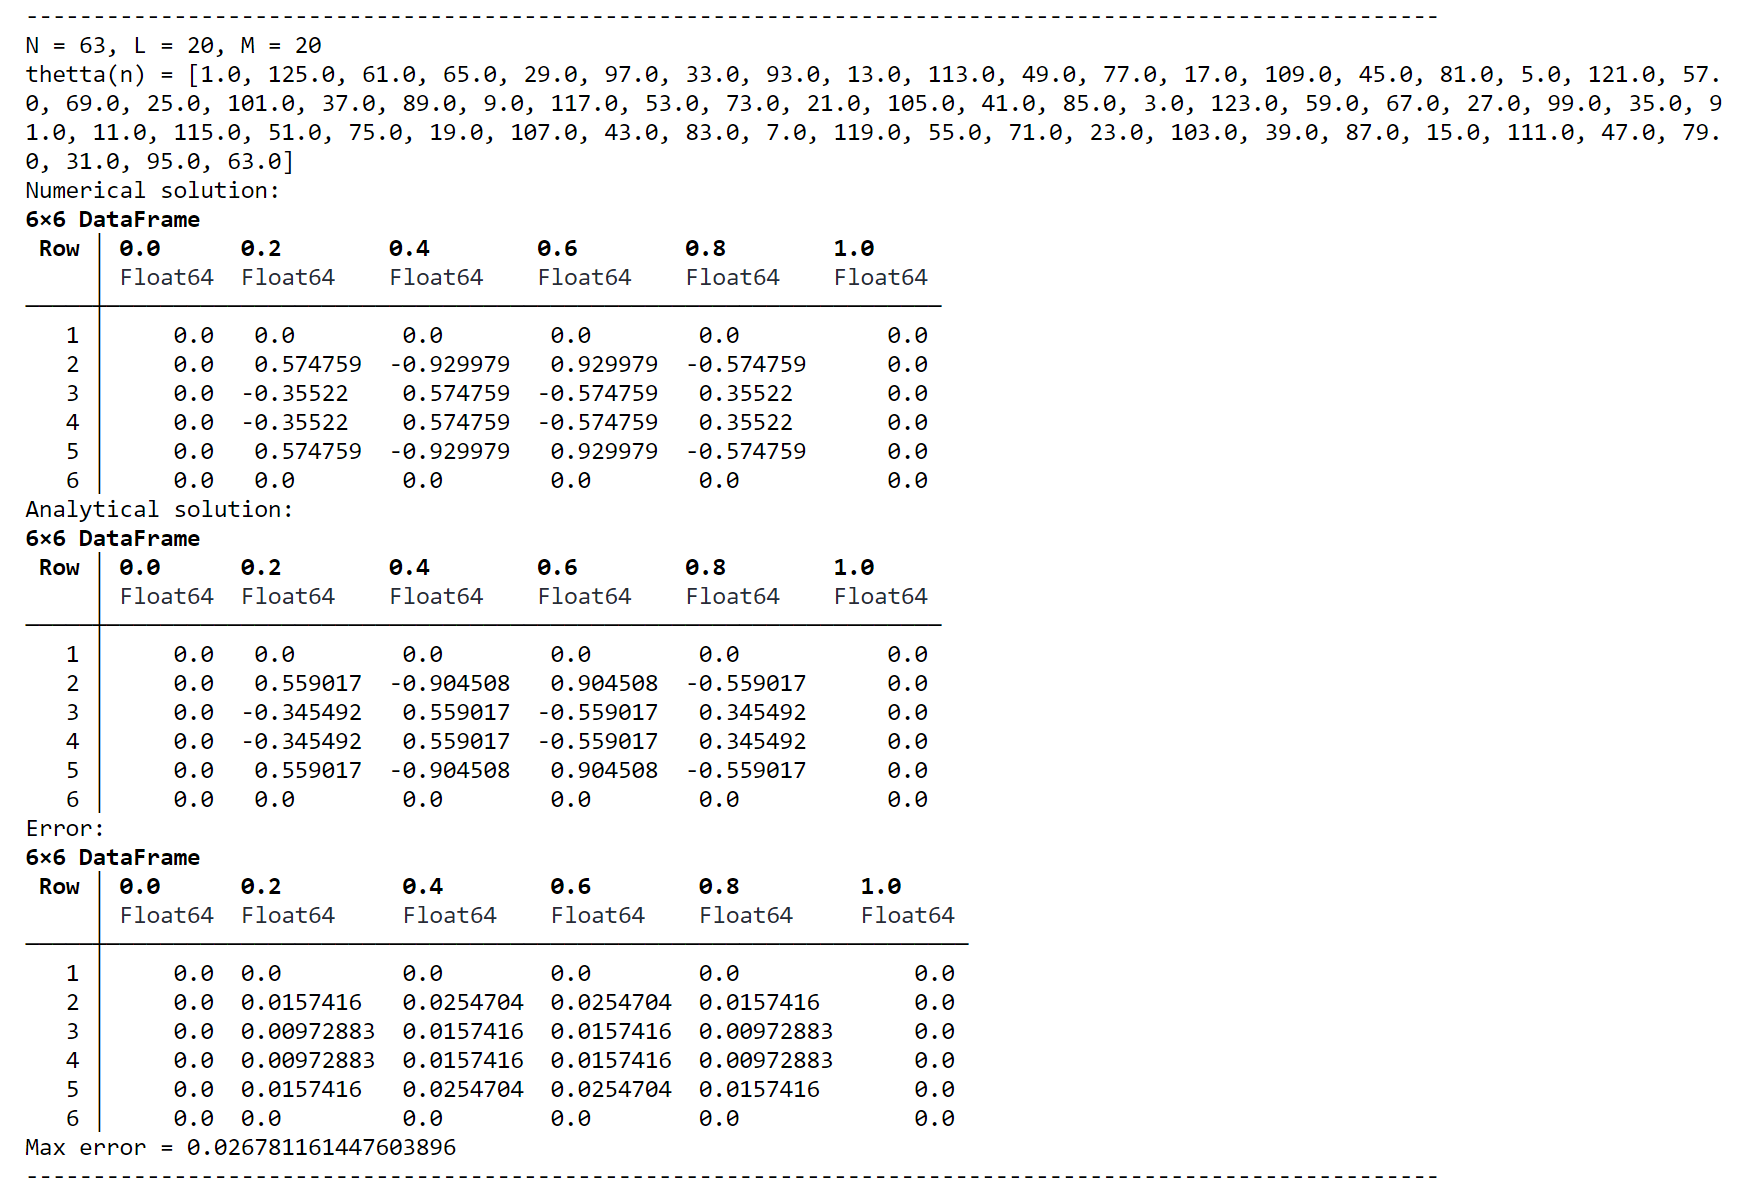
\includegraphics[width = 1.0\textwidth]{lab5_2.png}
\end{figure}

\begin{figure}[H]
	\centering
	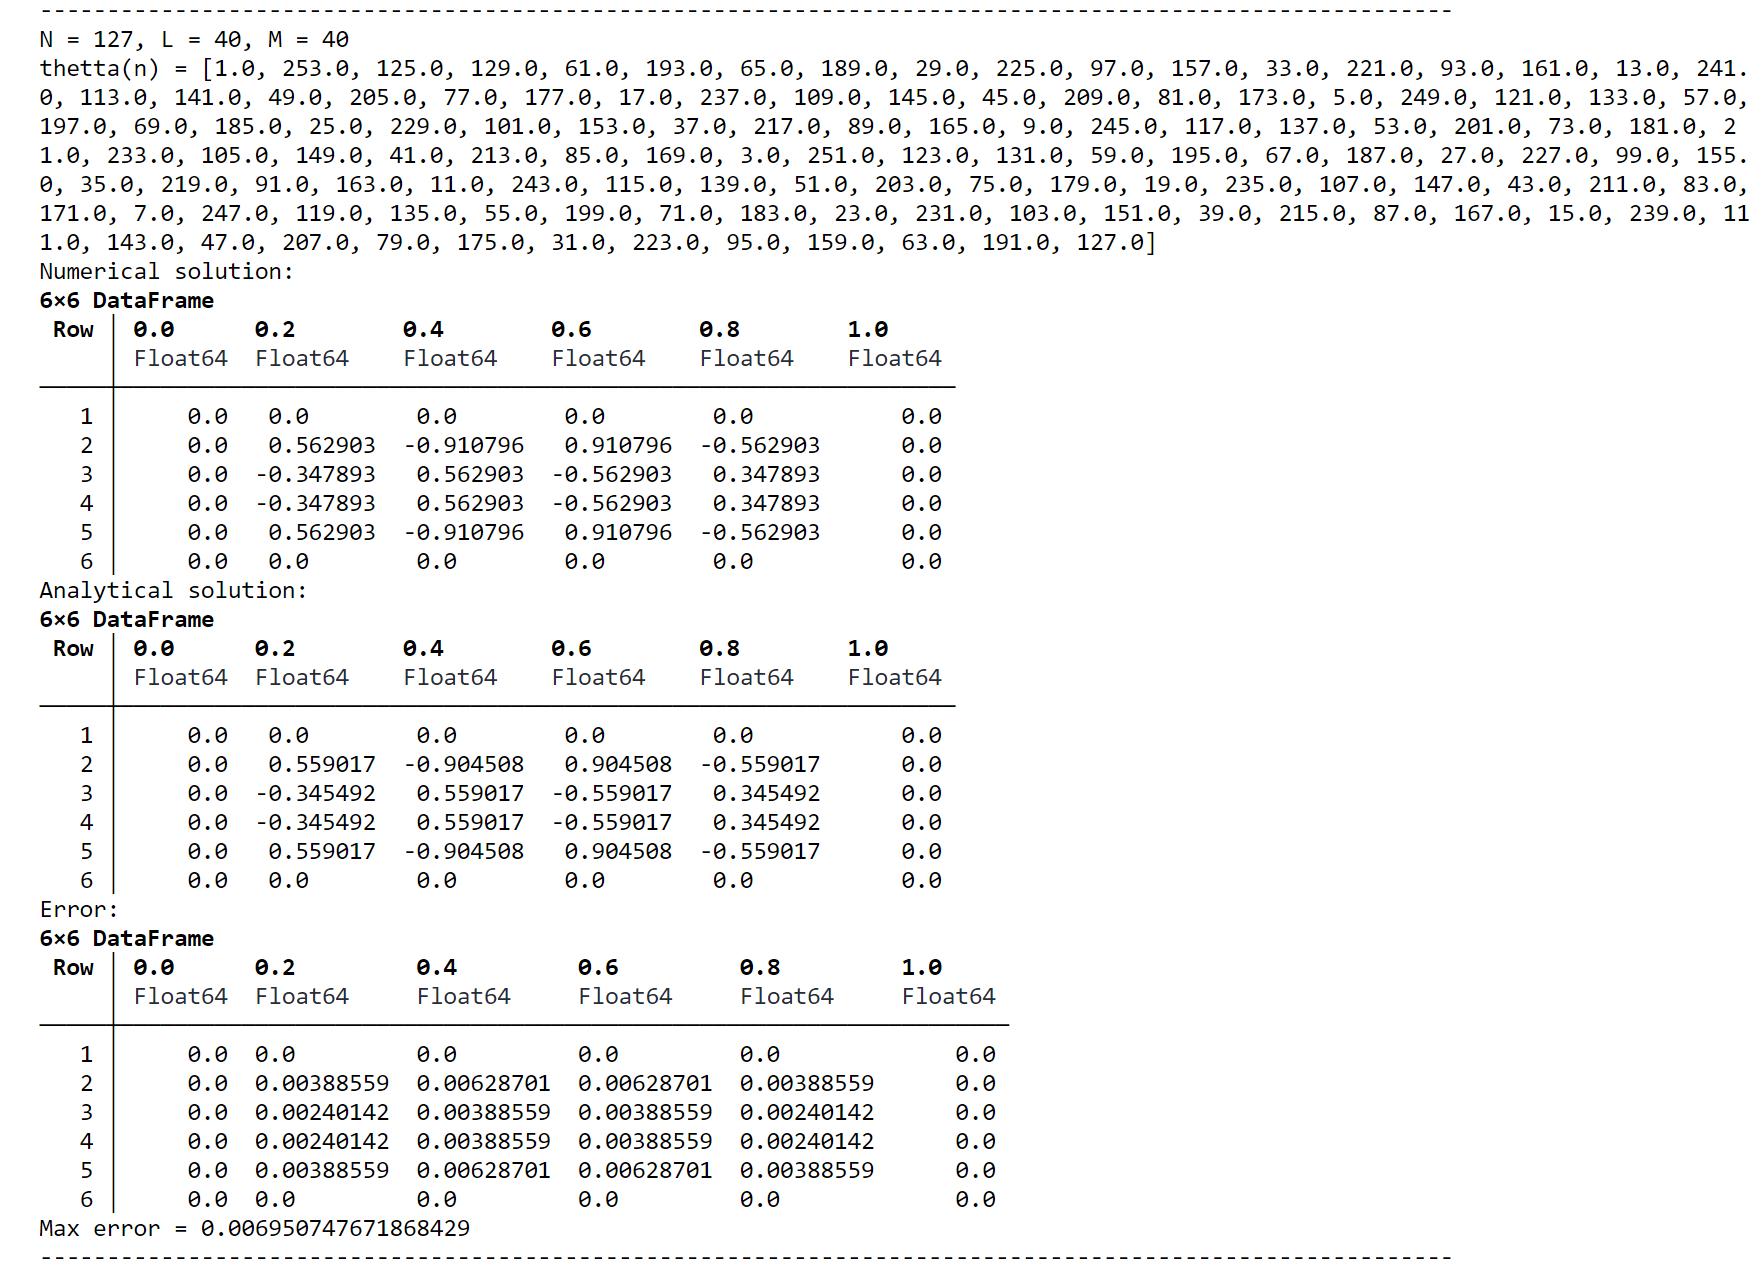
\includegraphics[width = 1.0\textwidth]{lab5_3.png}
\end{figure}

\begin{figure}[H]
	\centering
	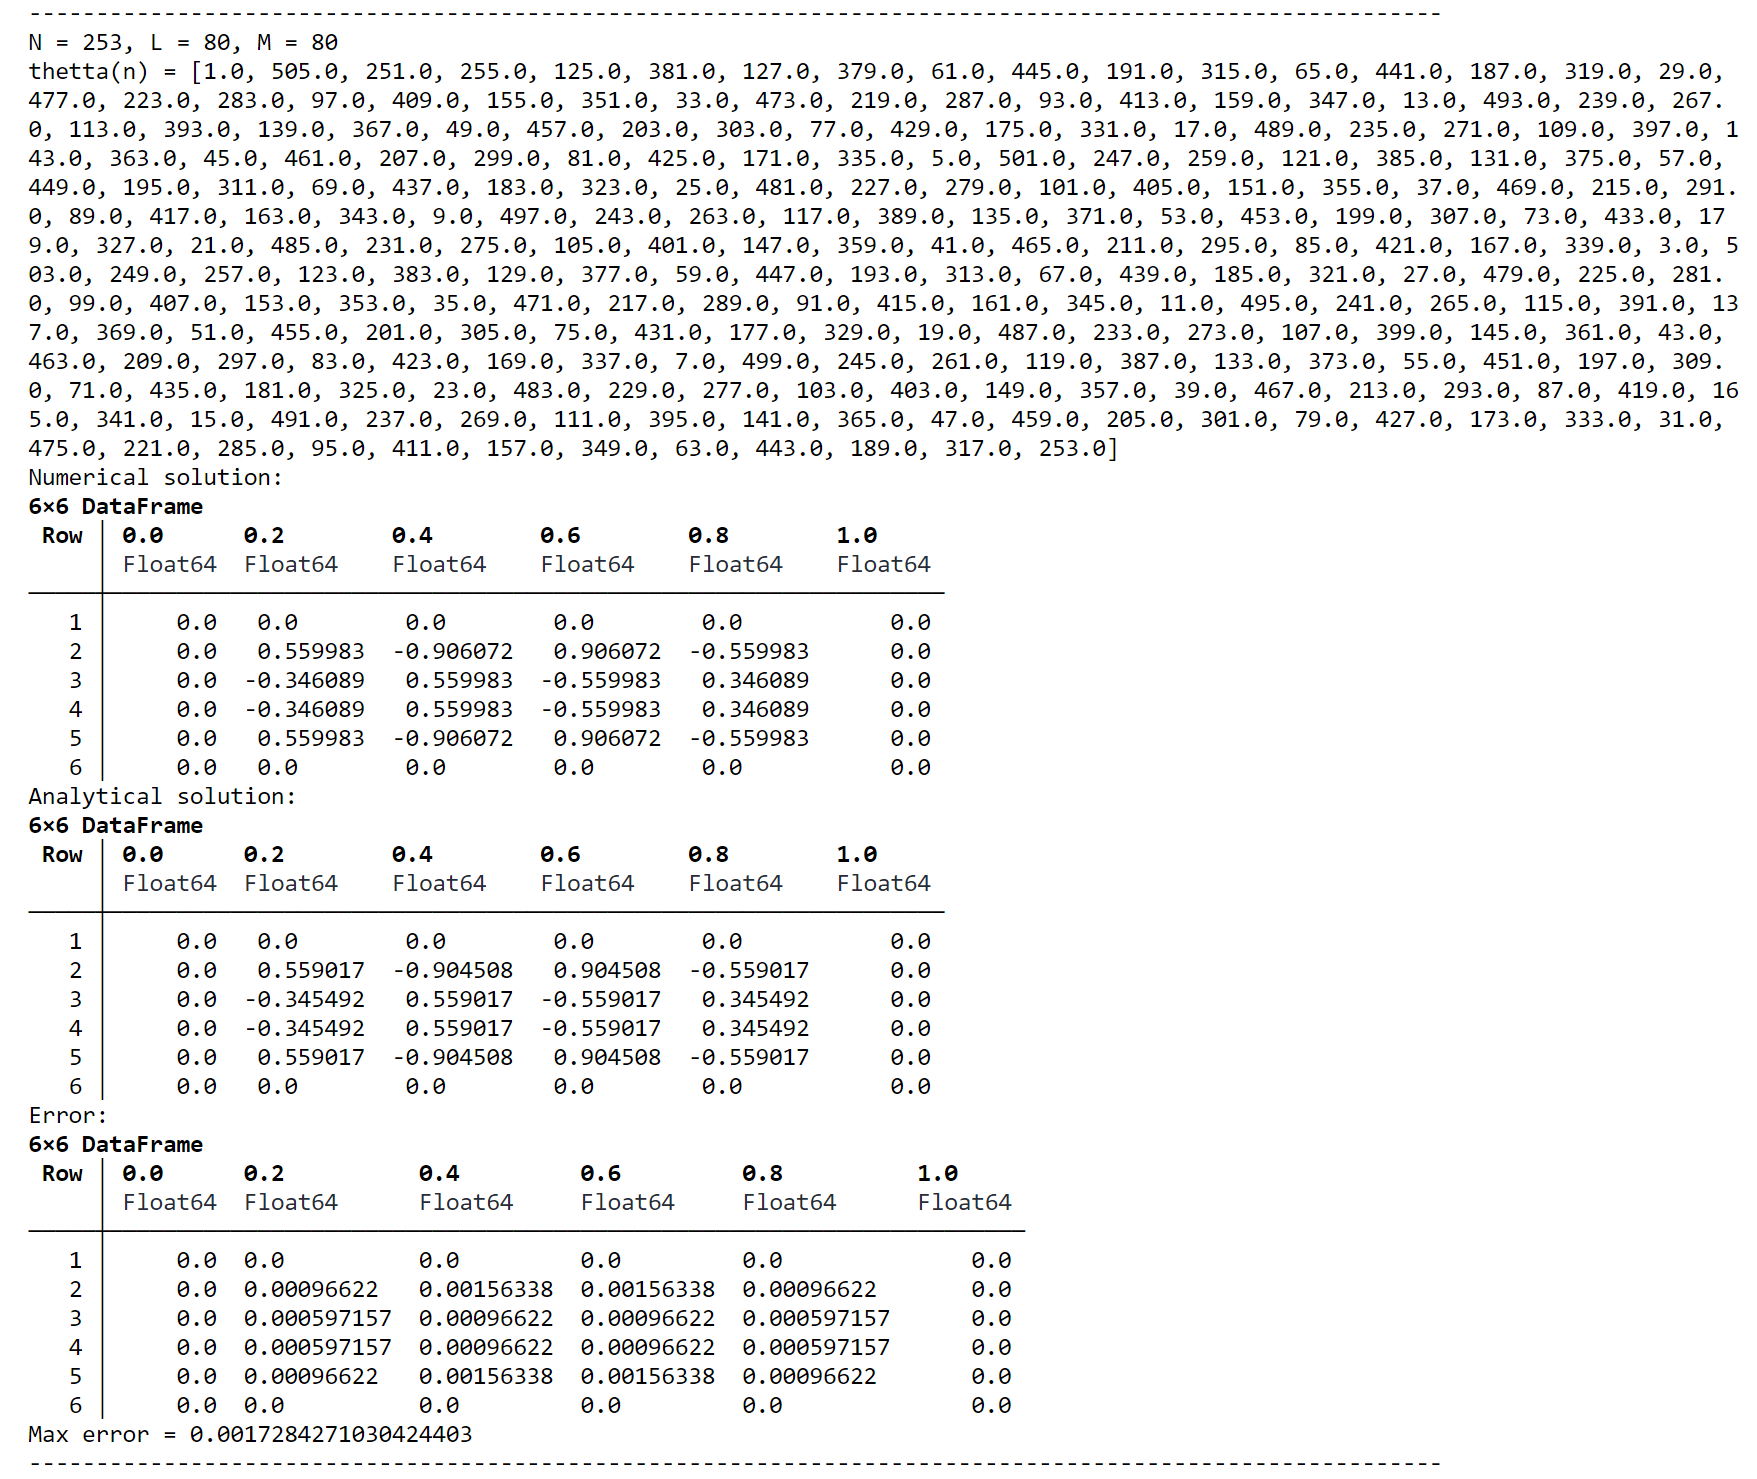
\includegraphics[width = 1.0\textwidth]{lab5_4.png}
\end{figure}

\begin{figure}[H]
	\centering
	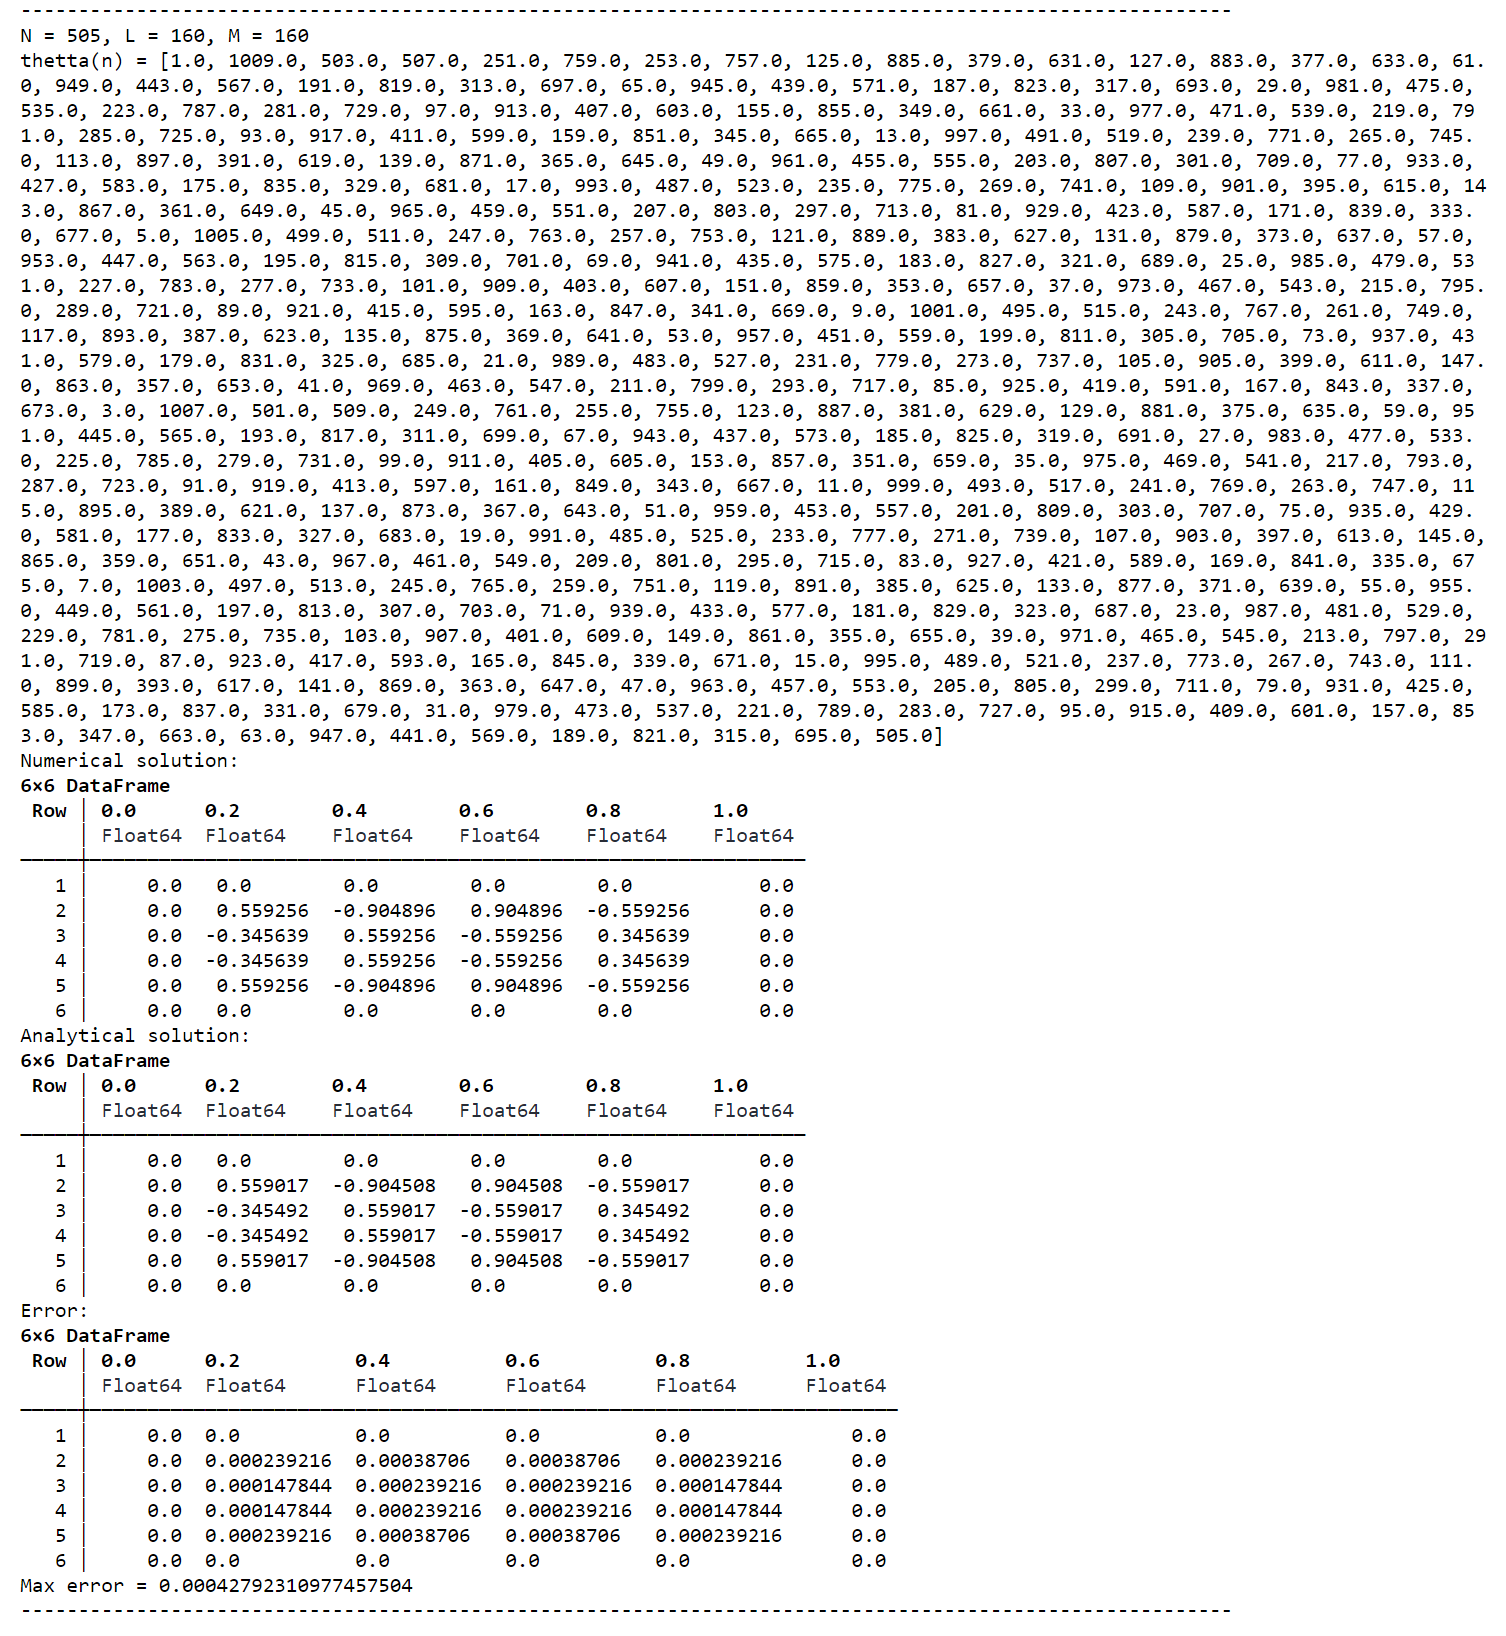
\includegraphics[width = 1.0\textwidth]{lab5_5.png}
\end{figure}

\begin{figure}[H]
	\centering
	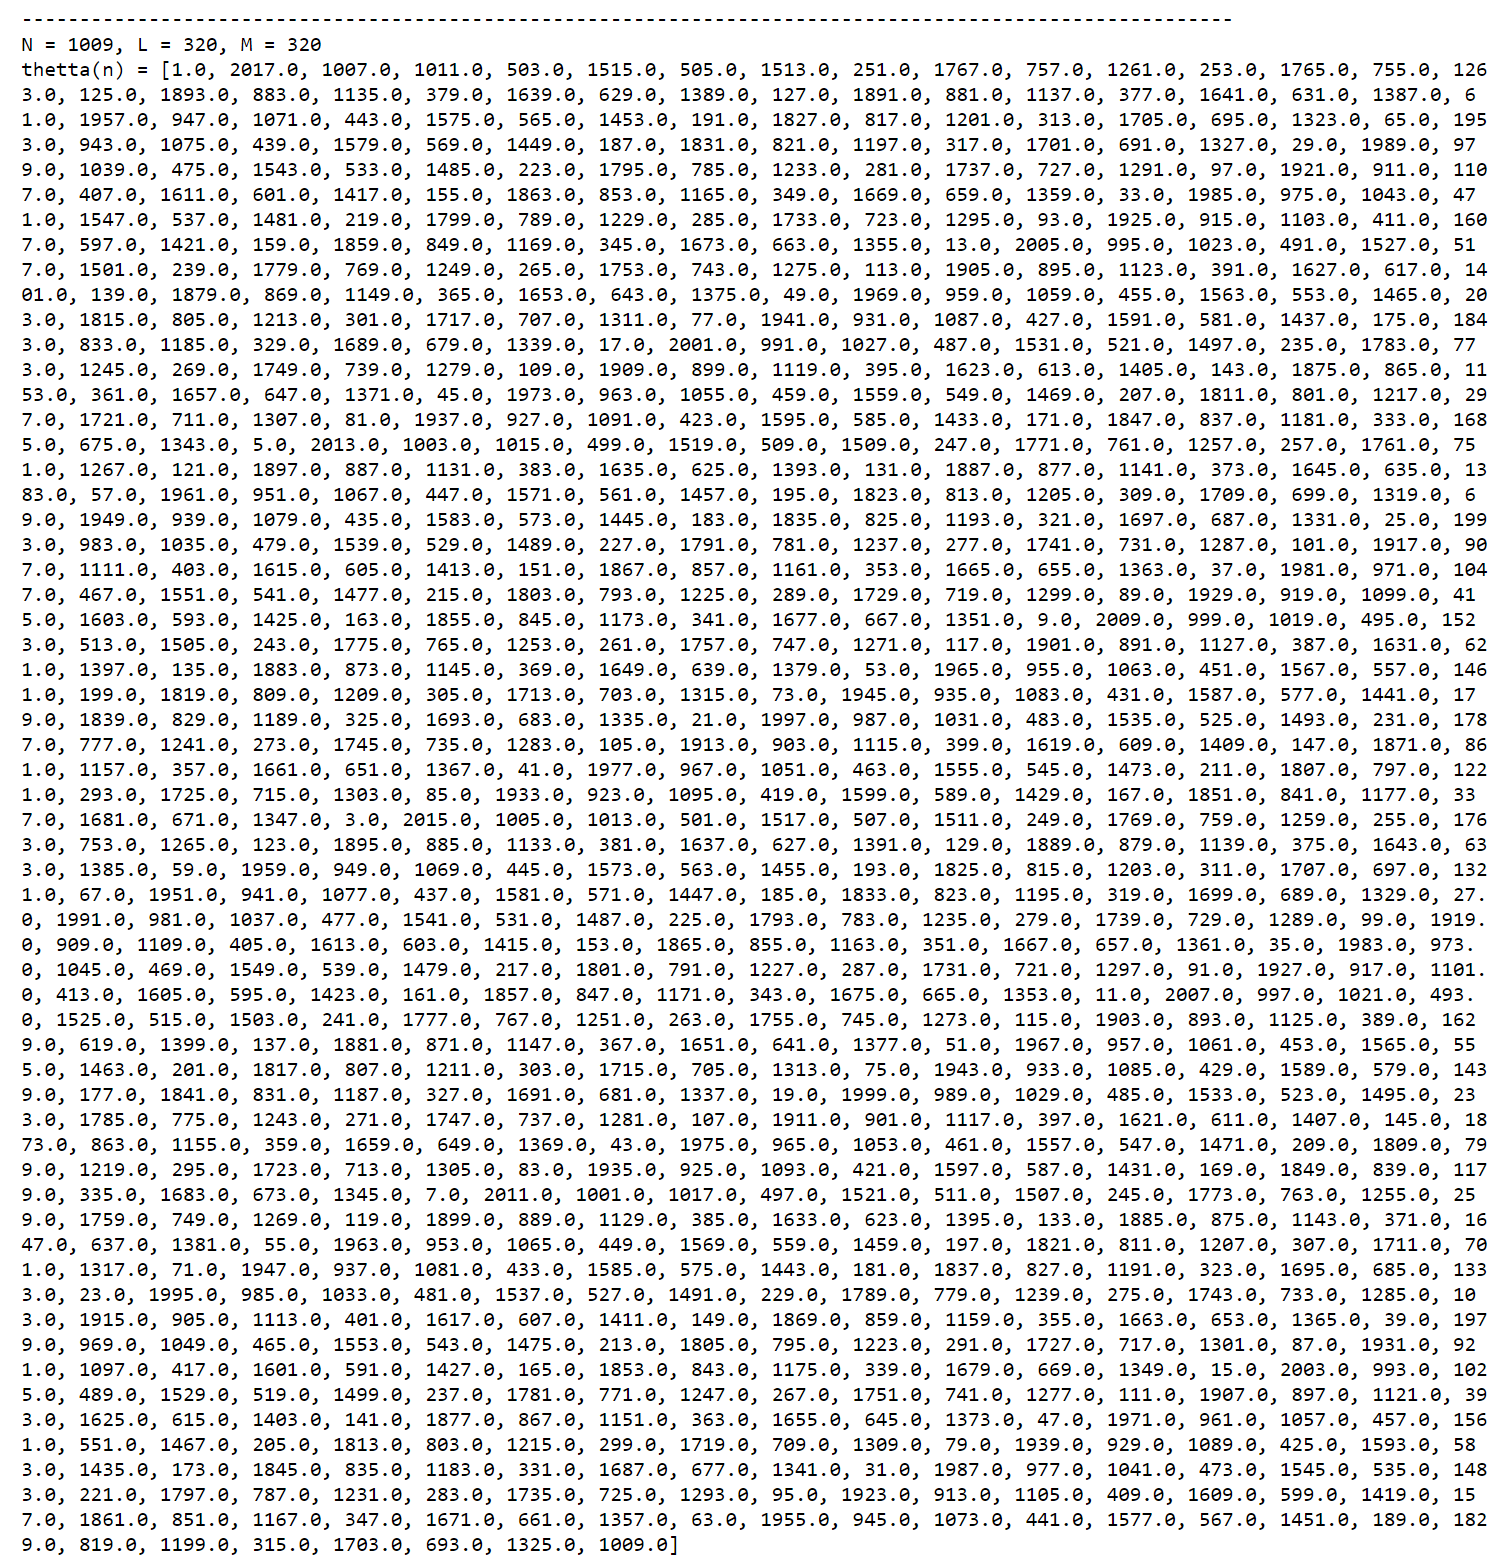
\includegraphics[width = 1.0\textwidth]{lab5_6_1.png}
\end{figure}

\begin{figure}[H]
	\centering
	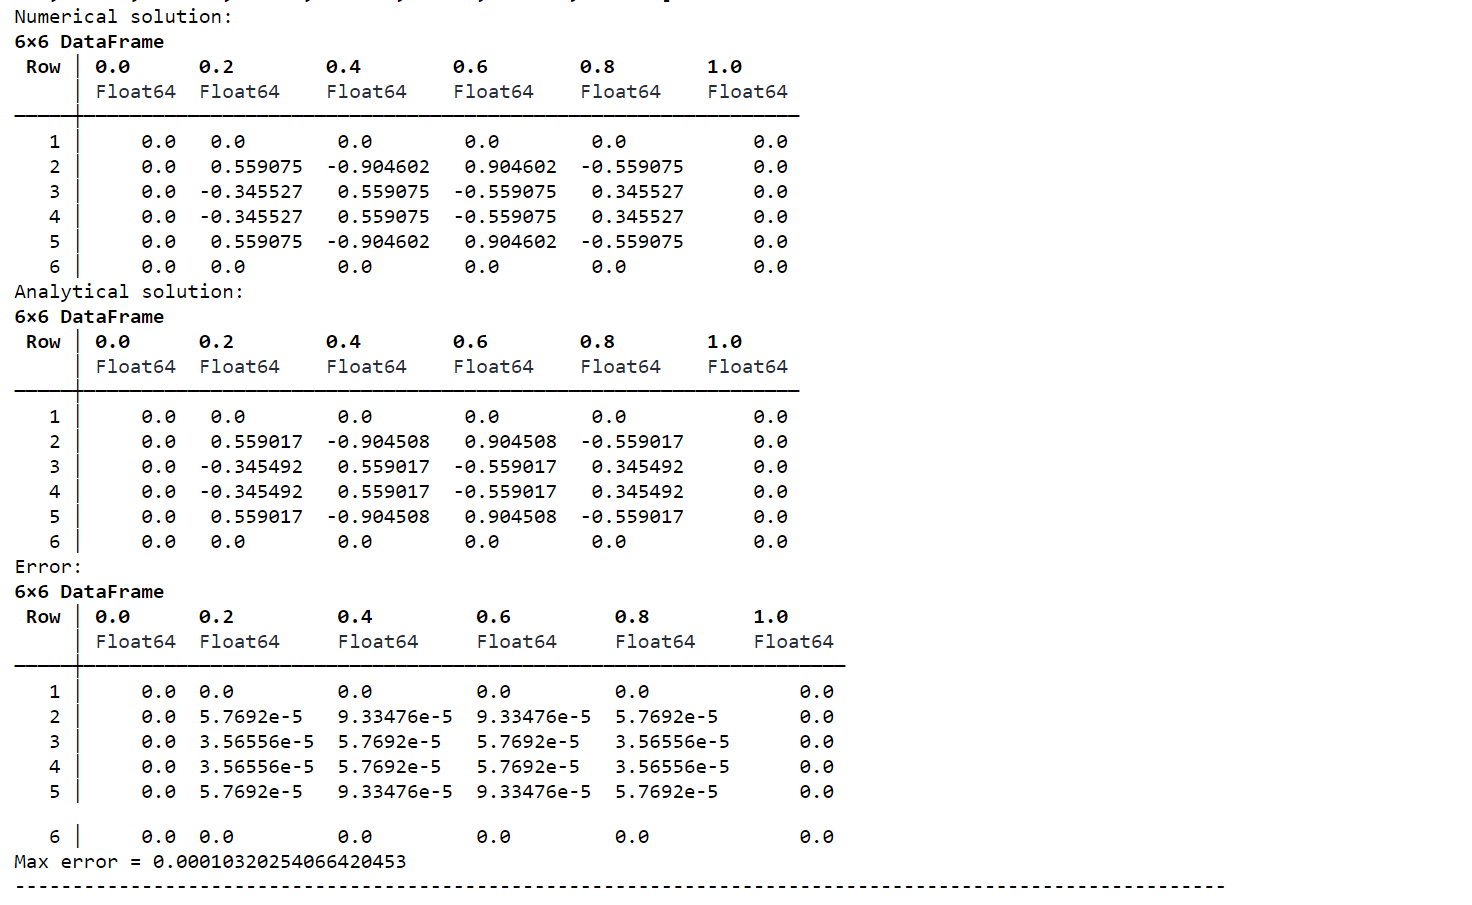
\includegraphics[width = 1.0\textwidth]{lab5_6_2.png}
\end{figure}

\subsection*{Результаты и обсуждения}
\noindent\rule{\textwidth}{1pt}
В данной работе представлена схема, по которой проводились численные расчеты, найдено аналитическое решение и ее след. Выявлен набор $\tau_n$ для каждой тройки N, L, M. Найдено численное решение для каждой тройки с учетом выбранного чебышевского набора, причем наблюдается устойчивость и сходимость решения на последовательно удваеваемых сетках. На последовательно удваеваемых сетках также наблюдается уменьшение ошибки примерно в 4 раза при уменьшении сетки вдвое по каждой оси.

\end{document}